% Generated by figures/ablation_figure.py -- do not edit by hand.
\begin{figure*}[t]
\centering
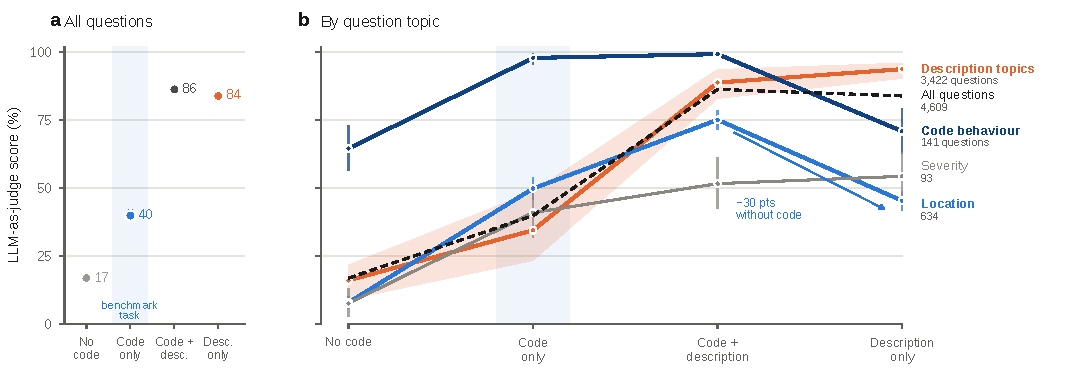
\includegraphics[width=\textwidth]{fig_ablation.pdf}
\caption{LLM-as-judge score of Gemma-4-31B on the same 999 test records (4,609 questions) with four inputs;
the shaded column is the benchmark task. (a)~All questions. (b)~By question topic. Orange: the six topics that the CVE description answers far better than
the code (vulnerability type, mechanism, fix, impact, exploitation and affected software), pooled (line) and their
range (band). Blue: the topics that need the code; removing the code from the
input lowers their scores by 30 (location) and
28 (code behaviour) points. Grey: severity,
which neither input answers well. Dashed: all questions. Vertical bars are 95\% bootstrap intervals over records;
Table~\ref{tab:ablation-topics} in the appendix gives every topic.}
\label{fig:ablation}
\end{figure*}
